\chapter{Background}

% Background to explain context and significance of the question we are addressing.

% What is PCG? (definition and explain with examples)
PCG is a family of algorithms that automatically and randomly generates synthetic media such as 3D models, textures, items, quests, levels and music~\cite[p.1]{pcg_in_games}.
Typically, this generation is achieved by combining manually designed assets with stochastic, yet controllable algorithms.
The algorithms are restricted by manually designed rules to only produce quality content, and utilize randomness within these constraints to generate diverse results~\cite{gamasutra}.
For instance, a correct PCG algorithm for car generation would always produce functional cars, but the resulting cars will still vary by configurable properties such as wheels, seats, size, engine, price, and name.

% History
In the early 1980s, PCG was primarily used in games as a workaround for the limited storage space in computers~\cite[p.4]{pcg_in_games}.
This workaround has lead to a whole new genre of games called \textit{roguelike} that is still thriving today \cite{roguelikes}.
However, in recent years PCG has gained traction for other reasons than small file sizes.

Populating large games with content is a labor-intensive process if done by hand, and PCG has been used to tackle this problem by speeding up development times and by producing new experiences for each playthrough.
For instance, the game \textit{Minecraft} \cite{minecraft} uses PCG to generate all of its procedural worlds (See figure \ref{fig:minecraft}).

\begin{figure}[h!]
  \centering

  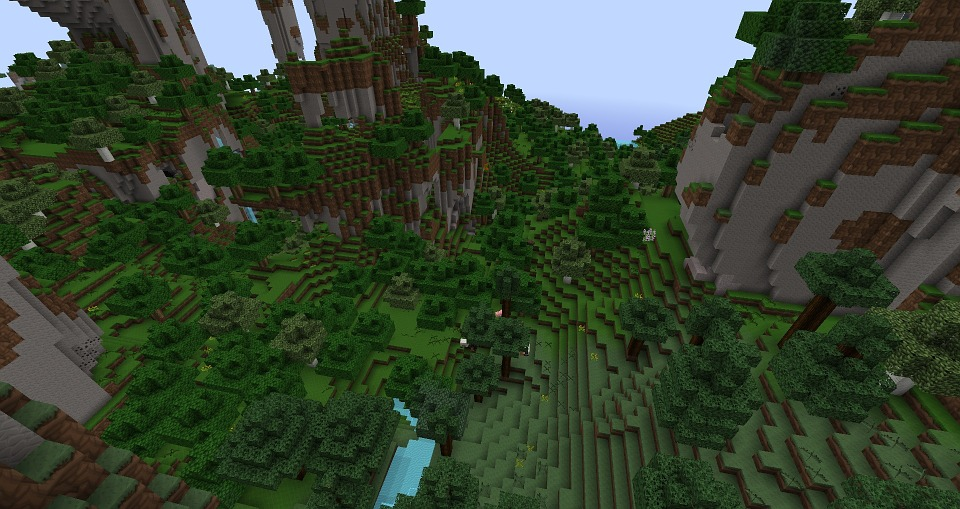
\includegraphics[width=0.8\textwidth]{figure/minecraft.jpg}
  \caption{Example of a pseudo-infinite world generated in Minecraft \cite{minecraft_img}.}

  \label{fig:minecraft}
\end{figure}

% Difference between offline and online generation
PCG can be performed either before or during runtime, in which case the generation is referred to as offline or online respectively \cite[p. 7-8]{pcg_in_games}.
Since online generation is performed while a user is interacting with the media, it is critical that any computations are light enough for the software to run smoothly and that all results produced are acceptable to the end-user.
Meanwhile, offline generation has typically significantly looser requirements since it is performed during the development process.
However, online generation has the crucial advantage of being able to dynamically adjust its generated content based on user interactions.

% Examples usages of offline generation
Offline is arguably the most common type of generation due to its broad definition and its loose restrictions.
It is commonly used to accelerate the work of artists by generating good candidates which artists can then manually refine, examples include the creation of landscape in \textit{Oblivion} \cite{elder_scrolls_iv}.
This approach is also the typical way software like SpeedTree \cite{speedtree} is used, and is the intended way to use the city generation software presented in this report.

% Examples usages of online generation
Online generation is also highly useful, but primarily in interactive media like video games.
Some of its commercial applications include the
\begin{easylist}
  @ pseudo-infinite worlds in \textit{Minecraft} \cite{minecraft} and \textit{No Man's Sky} \cite{no_man_sky}.
  @ unpredictable level layouts in the \textit{Civilization} \cite{civilization} and \textit{Diablo} \cite{diablo} series.
  @ procedural weapons in \textit{Dead Cells} \cite{dead_cells}, \textit{Terraria} \cite{terraria}, and \textit{Borderlands} \cite{borderlands}.
  @ procedural creatures in \textit{Spore} \cite{spore} and \textit{No Man's Sky} \cite{no_man_sky}.
  @ dynamic difficulty found in \textit{Left 4 Dead 2} \cite{left_4_dead_2}.
\end{easylist}
There is of course also \textit{Dwarf Fortress} \cite{dwarf_fortress} which generates everything imaginable, from world history to character personalities.
All of these games benefit from improved replayability and unpredictability with online generation, albeit by different means and to various degrees.
The prime examples being \textit{Minecraft} and \textit{Terraria} who both extensively use PCG throughout their game mechanics, and who both have received outstanding critical and commercial success \cite{minecraft_reviews} \cite{minecraft_commercial} \cite{terraria_reviews} \cite{terraria_commercial}.
Although PCG itself is not a recipe for success, as seen with the launch of \textit{No Man's Sky} \cite{no_man_sky_launch}, but even that game made a comeback \cite{no_man_sky_comeback}.

% Tied to games, but movies as well.
Nowadays, the terms \textit{PCG} and \textit{procedural generation} are heavily tied to games, with some even describing PCG as ``the algorithmic creation of game content'' \cite[p.1]{pcg_in_games}.
Although games have seen several benefits from PCG, such as improved variation and replayability, it is worth noting that the field has seen extensive use in other mediums as well.
One such medium being film.
For example, the software package MASSIVE was used throughout the \textit{Lord of the Rings} trilogy to generate crowd-related visual effects \cite{massive}, and generation of vegetation using SpeedTree has become an industry standard \cite{speedtree_cinema}.
% Nonetheless, PCG is rarely marketed in the film industry.
Nonetheless, most PCG research seem to target games.
